% Options for packages loaded elsewhere
\PassOptionsToPackage{unicode}{hyperref}
\PassOptionsToPackage{hyphens}{url}
\PassOptionsToPackage{dvipsnames,svgnames,x11names}{xcolor}
%
\documentclass[
  letterpaper,
  DIV=11,
  numbers=noendperiod]{scrartcl}

\usepackage{amsmath,amssymb}
\usepackage{iftex}
\ifPDFTeX
  \usepackage[T1]{fontenc}
  \usepackage[utf8]{inputenc}
  \usepackage{textcomp} % provide euro and other symbols
\else % if luatex or xetex
  \usepackage{unicode-math}
  \defaultfontfeatures{Scale=MatchLowercase}
  \defaultfontfeatures[\rmfamily]{Ligatures=TeX,Scale=1}
\fi
\usepackage{lmodern}
\ifPDFTeX\else  
    % xetex/luatex font selection
\fi
% Use upquote if available, for straight quotes in verbatim environments
\IfFileExists{upquote.sty}{\usepackage{upquote}}{}
\IfFileExists{microtype.sty}{% use microtype if available
  \usepackage[]{microtype}
  \UseMicrotypeSet[protrusion]{basicmath} % disable protrusion for tt fonts
}{}
\makeatletter
\@ifundefined{KOMAClassName}{% if non-KOMA class
  \IfFileExists{parskip.sty}{%
    \usepackage{parskip}
  }{% else
    \setlength{\parindent}{0pt}
    \setlength{\parskip}{6pt plus 2pt minus 1pt}}
}{% if KOMA class
  \KOMAoptions{parskip=half}}
\makeatother
\usepackage{xcolor}
\setlength{\emergencystretch}{3em} % prevent overfull lines
\setcounter{secnumdepth}{-\maxdimen} % remove section numbering
% Make \paragraph and \subparagraph free-standing
\ifx\paragraph\undefined\else
  \let\oldparagraph\paragraph
  \renewcommand{\paragraph}[1]{\oldparagraph{#1}\mbox{}}
\fi
\ifx\subparagraph\undefined\else
  \let\oldsubparagraph\subparagraph
  \renewcommand{\subparagraph}[1]{\oldsubparagraph{#1}\mbox{}}
\fi


\providecommand{\tightlist}{%
  \setlength{\itemsep}{0pt}\setlength{\parskip}{0pt}}\usepackage{longtable,booktabs,array}
\usepackage{calc} % for calculating minipage widths
% Correct order of tables after \paragraph or \subparagraph
\usepackage{etoolbox}
\makeatletter
\patchcmd\longtable{\par}{\if@noskipsec\mbox{}\fi\par}{}{}
\makeatother
% Allow footnotes in longtable head/foot
\IfFileExists{footnotehyper.sty}{\usepackage{footnotehyper}}{\usepackage{footnote}}
\makesavenoteenv{longtable}
\usepackage{graphicx}
\makeatletter
\def\maxwidth{\ifdim\Gin@nat@width>\linewidth\linewidth\else\Gin@nat@width\fi}
\def\maxheight{\ifdim\Gin@nat@height>\textheight\textheight\else\Gin@nat@height\fi}
\makeatother
% Scale images if necessary, so that they will not overflow the page
% margins by default, and it is still possible to overwrite the defaults
% using explicit options in \includegraphics[width, height, ...]{}
\setkeys{Gin}{width=\maxwidth,height=\maxheight,keepaspectratio}
% Set default figure placement to htbp
\makeatletter
\def\fps@figure{htbp}
\makeatother

\KOMAoption{captions}{tableheading}
\makeatletter
\makeatother
\makeatletter
\makeatother
\makeatletter
\@ifpackageloaded{caption}{}{\usepackage{caption}}
\AtBeginDocument{%
\ifdefined\contentsname
  \renewcommand*\contentsname{Table of contents}
\else
  \newcommand\contentsname{Table of contents}
\fi
\ifdefined\listfigurename
  \renewcommand*\listfigurename{List of Figures}
\else
  \newcommand\listfigurename{List of Figures}
\fi
\ifdefined\listtablename
  \renewcommand*\listtablename{List of Tables}
\else
  \newcommand\listtablename{List of Tables}
\fi
\ifdefined\figurename
  \renewcommand*\figurename{Figure}
\else
  \newcommand\figurename{Figure}
\fi
\ifdefined\tablename
  \renewcommand*\tablename{Table}
\else
  \newcommand\tablename{Table}
\fi
}
\@ifpackageloaded{float}{}{\usepackage{float}}
\floatstyle{ruled}
\@ifundefined{c@chapter}{\newfloat{codelisting}{h}{lop}}{\newfloat{codelisting}{h}{lop}[chapter]}
\floatname{codelisting}{Listing}
\newcommand*\listoflistings{\listof{codelisting}{List of Listings}}
\makeatother
\makeatletter
\@ifpackageloaded{caption}{}{\usepackage{caption}}
\@ifpackageloaded{subcaption}{}{\usepackage{subcaption}}
\makeatother
\makeatletter
\@ifpackageloaded{tcolorbox}{}{\usepackage[skins,breakable]{tcolorbox}}
\makeatother
\makeatletter
\@ifundefined{shadecolor}{\definecolor{shadecolor}{rgb}{.97, .97, .97}}
\makeatother
\makeatletter
\makeatother
\makeatletter
\makeatother
\ifLuaTeX
  \usepackage{selnolig}  % disable illegal ligatures
\fi
\IfFileExists{bookmark.sty}{\usepackage{bookmark}}{\usepackage{hyperref}}
\IfFileExists{xurl.sty}{\usepackage{xurl}}{} % add URL line breaks if available
\urlstyle{same} % disable monospaced font for URLs
\hypersetup{
  pdftitle={West Nile Virus Blog Post},
  colorlinks=true,
  linkcolor={blue},
  filecolor={Maroon},
  citecolor={Blue},
  urlcolor={Blue},
  pdfcreator={LaTeX via pandoc}}

\title{West Nile Virus Blog Post}
\author{}
\date{}

\begin{document}
\maketitle
\ifdefined\Shaded\renewenvironment{Shaded}{\begin{tcolorbox}[interior hidden, sharp corners, boxrule=0pt, borderline west={3pt}{0pt}{shadecolor}, frame hidden, breakable, enhanced]}{\end{tcolorbox}}\fi

\hypertarget{west-nile-virus-incidence-in-pennsylvania-mosquitoes}{%
\section{West Nile Virus Incidence in Pennsylvania
Mosquitoes}\label{west-nile-virus-incidence-in-pennsylvania-mosquitoes}}

\hypertarget{introduction}{%
\subsection{Introduction:}\label{introduction}}

In 2018, Pennsylvania experienced one of it's worst West Nile Virus
(WNV) outbreaks in 15 years, resulting in around 72 cases reported in
humans and three deaths from the virus
\href{https://www.publicopiniononline.com/story/news/2018/10/09/pennsylvanias-worst-outbreak-west-nile-virus-15-years/1580572002/}{1}.
According to the Pennsylvania Department of Environmental Protection
(DEP), West Nile Virus first entered the state in 2000 and since then,
multiple state departments(Department of Environmental Protection,
Department of Agriculture, and Department of Health) have embarked on a
joint effort to manage the mosquito population to help reduce the risk
of the virus and educate the public on how to reduce their risk of
infection thought Integrated Pest Management
\href{https://www.dep.pa.gov/Business/ProgramIntegration/Vector-Management/Mosquitoes/Pages/default.aspx}{2}.

\hypertarget{what-is-west-nile-virus}{%
\subsection{What is West Nile Virus?:}\label{what-is-west-nile-virus}}

West Nile Virus is a vector born disease that cycles itself through
birds (hosts) and mosquitoes (vectors), where a bird infected by WNV
from a mosquito can in turn infect an uninfected mosquito who then bites
that infected
bird\href{https://www.dep.pa.gov/Business/ProgramIntegration/Vector-Management/Mosquitoes/Pages/default.aspx}{2}.
From there, WNV transmits itself to humans and other mammals. In
Pennsylvania, the primary concern for WNV transmission in non-human
animals are horses and wild game, particularly birds.

\hypertarget{area-of-interest}{%
\subsection{Area of Interest:}\label{area-of-interest}}

Philadelphia has ranked among the top cities for both mosquito rates and
WNV cases in
humans{[}1{]}(\url{https://www.publicopiniononline.com/story/news/2018/10/09/pennsylvanias-worst-outbreak-west-nile-virus-15-years/1580572002/}\href{https://www.publicopiniononline.com/story/news/2018/10/09/pennsylvanias-worst-outbreak-west-nile-virus-15-years/1580572002/}{){[}3{]}(https://www.inquirer.com/science/climate/mosquitos-climate-change-climate-central-global-warming-philadelphia-allentown-atlantic-city-zika-20200804.html}\href{https://www.inquirer.com/science/climate/mosquitos-climate-change-climate-central-global-warming-philadelphia-allentown-atlantic-city-zika-20200804.html}{3}).
Mosquitoes season ranges from around March to late October when
temperatures are warmer, typically seeing spikes in July. But due to
climate change, mosquito season is lasting longer, increasing the
potential for exposure to WNV
\href{\%5Bhttps://www.inquirer.com/science/climate/mosquitos-climate-change-climate-central-global-warming-philadelphia-allentown-atlantic-city-zika-20200804.htmlhttps://www.inquirer.com/science/climate/mosquitos-climate-change-climate-central-global-warming-philadelphia-allentown-atlantic-city-zika-20200804.html\%5D(https://www.inquirer.com/science/climate/mosquitos-climate-change-climate-central-global-warming-philadelphia-allentown-atlantic-city-zika-20200804.html)}{3}.
While an increase in mosquitoes does not inherently mean an increase in
disease cases, investigating the link could be worthwhile.

\hypertarget{data}{%
\subsection{Data:}\label{data}}

The data for this study was collected from:

{[}The Pennsylvania Department of Environmental
Protection{]}(\url{https://files.dep.state.pa.us/Water/WNV/MosquitoTestingData/})

and the {[}Pennsylvania State
Climatologist{]}(\url{https://climate.met.psu.edu/data/})

\hypertarget{research-question}{%
\subsection{Research Question:}\label{research-question}}

What is the impact of temperature and relative humidity on West Nile
Virus test results in Philadelphia mosquitoes?

\hypertarget{analysis}{%
\section{Analysis}\label{analysis}}

To begin the exploration into my analysis, I first conducted basic data
manipulation including cleaning the names of the data though
\texttt{janitor}, using \texttt{subset()} to to find data only within
Philadelphia, and using \texttt{merge()} to combine the Philadelphia
subset and the weather data. Additionally, to conduct my
\textbf{t-test}, the test result values ``POS'' and ``NEG'' were
converted to factors from character values using \texttt{as.factor()}.
For the \textbf{time series analysis}, the ``count'' column, containing
the counts of mosquitoes was aggregated by the date of collection column
renamed to ``date''. \texttt{aggregate()} was used to find the sum of
mosquito counts per day, since there were multiple collections
documented on the same day over the testing period. For \textbf{spatial
interpolation and kriging}, the entire 2018 data set was used, and since
there were multiple collections taken at the same location
\texttt{arrange()} and \texttt{distinct()} were used to organize the
rows and keep rows with only unique values for ``longitude'' and
``latitude.''

\hypertarget{exploratory-plotting}{%
\subsection{Exploratory Plotting}\label{exploratory-plotting}}

The following plots were used to discover potential trends in the data
before conducting further analysis. First, I created two violin box
plots (Fig. 1 and Fig. 2) to understand the visual distribution of both
temperature and relative humidity on mosquito test results. The
exploration for temperature shows a potential connection between test
results, however the exploration for relative humidity shows there is
potentially little relation.

\begin{figure}

{\centering 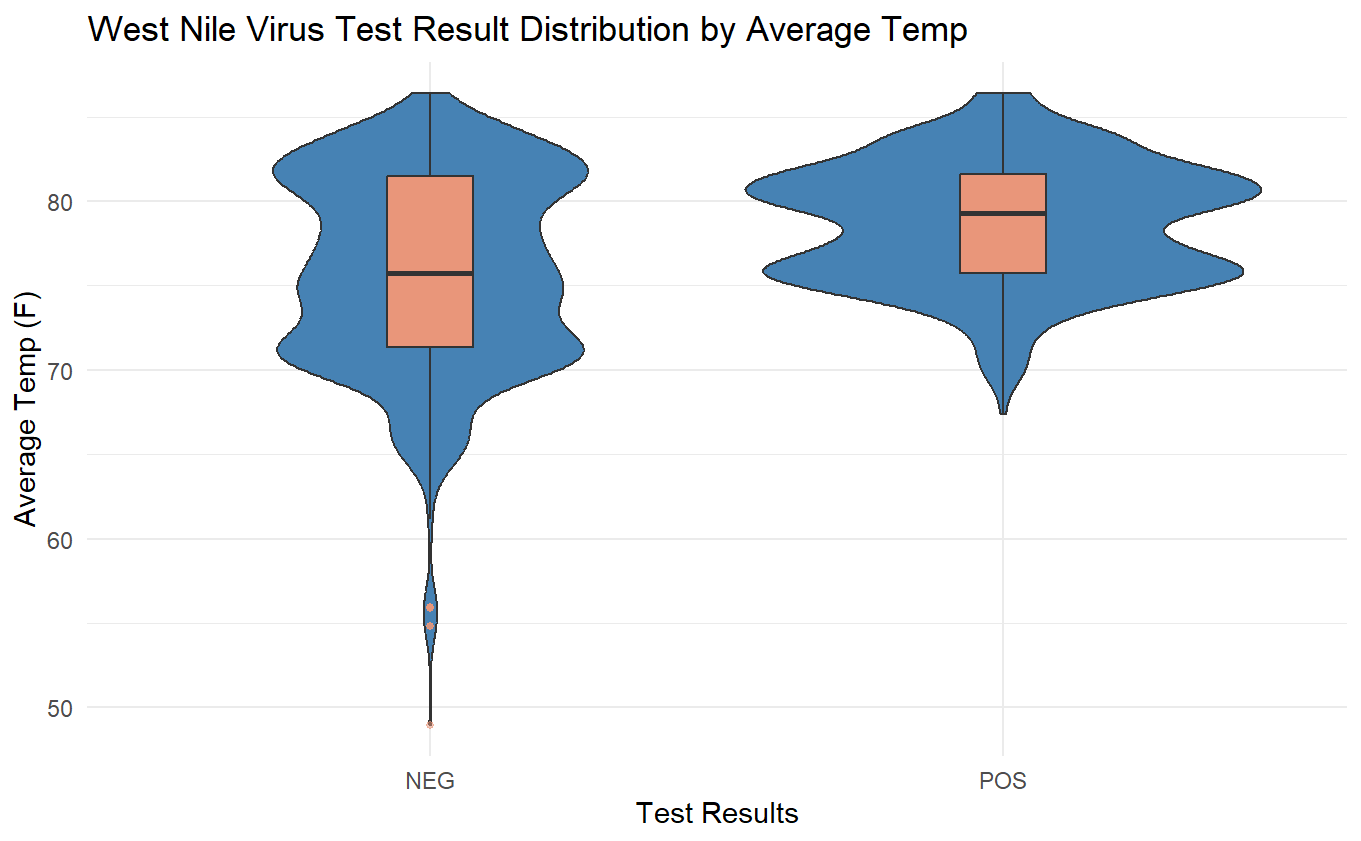
\includegraphics[width=8.33333in,height=\textheight]{images/temp_dist.png}

}

\caption{Fig. 1 Density of rates of positive and negative test results
for West Nile Virus in Mosquitos by average temperature. Temperature
data was collected as a daily average and is in Farenheit}

\end{figure}

\begin{figure}

{\centering 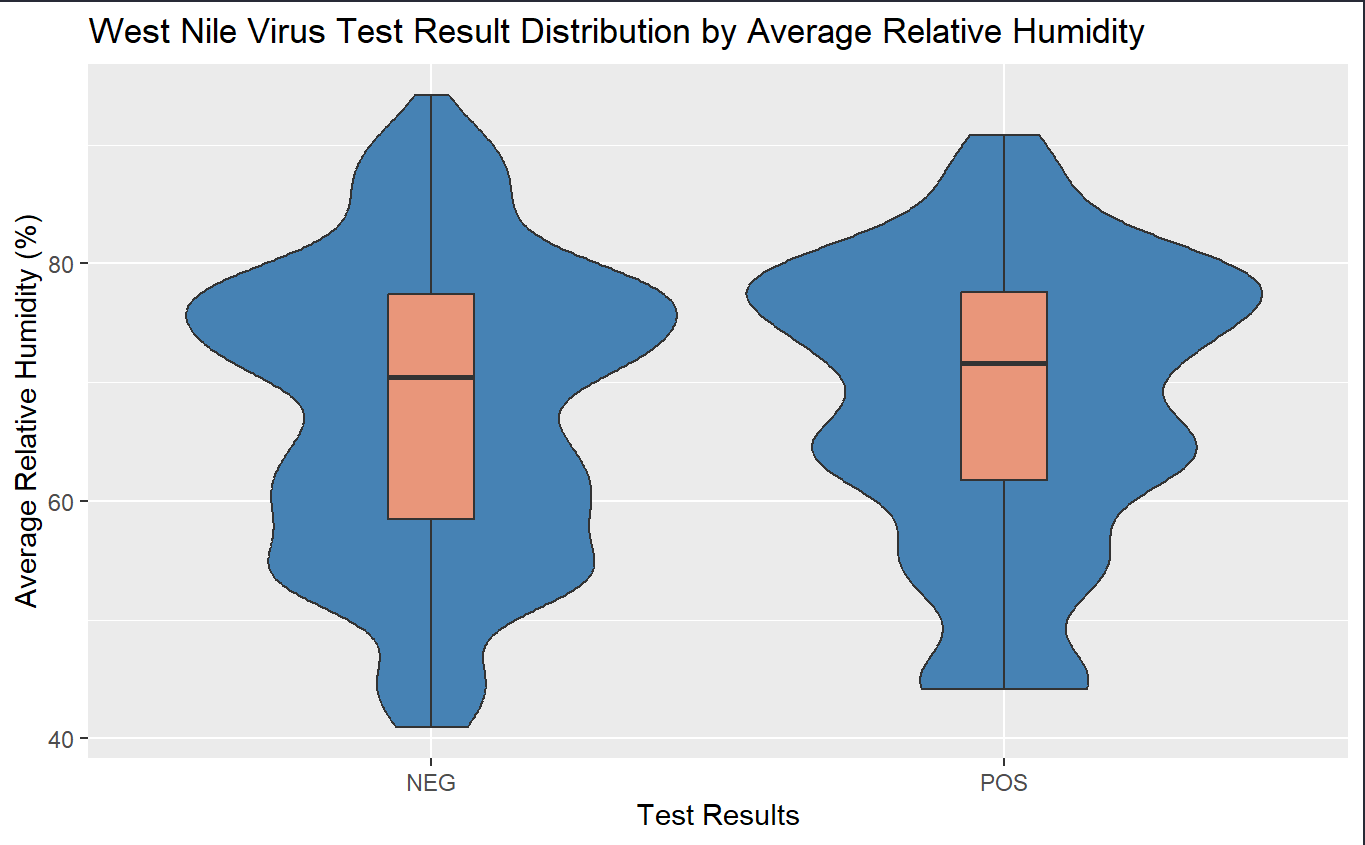
\includegraphics[width=8.33333in,height=\textheight]{images/rh_dist.png}

}

\caption{Fig. 2 Density rates of positive and negative test results for
West Nile Virus in Mosquitoes by Relative Humidity. Relative humidity
was collected as a daily average and is measured in percent}

\end{figure}

\hypertarget{hypothesis-testing}{%
\subsection{Hypothesis Testing}\label{hypothesis-testing}}

Since my primary research question is to explore if there is any
relationship between temperature and relative humidity and the test
results of mosquitoes, conducting a hypothesis test was my first method
of analysis. Where:

\textbf{\emph{Null Hypothesis: There is no difference in WNV test
results based on temperature/relative humidity}}

\textbf{\emph{Alternative Hypothesis:}} \textbf{\emph{There is a
difference in WNV test results based on temperature/relative humidity.}}

A hypothesis test was conducted on both temperature and relative
humidity. The results of the summary are as follows

\begin{figure}

{\centering 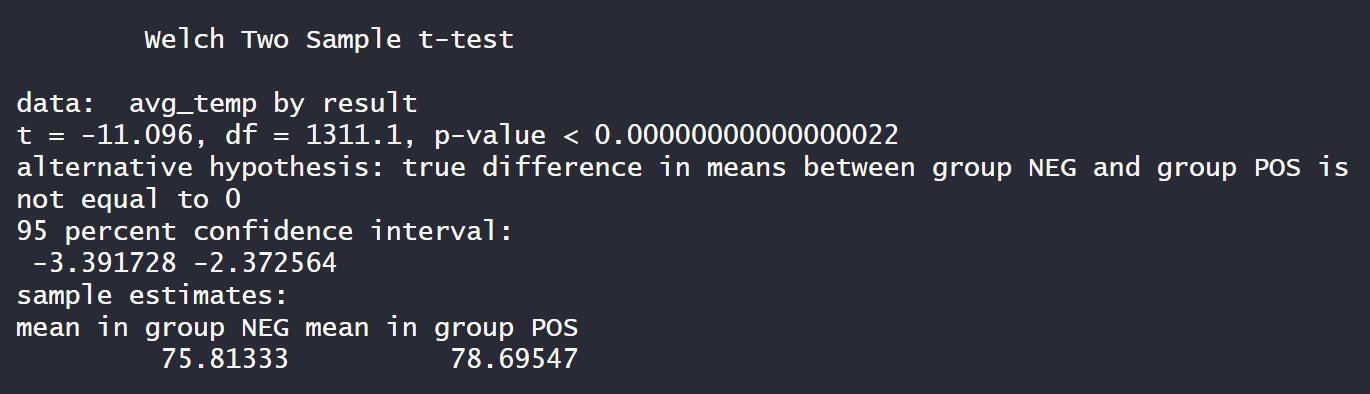
\includegraphics{images/Screenshot 2023-12-15 162119.png}

}

\caption{t-test conducted on average temperature and test results}

\end{figure}

\begin{figure}

{\centering 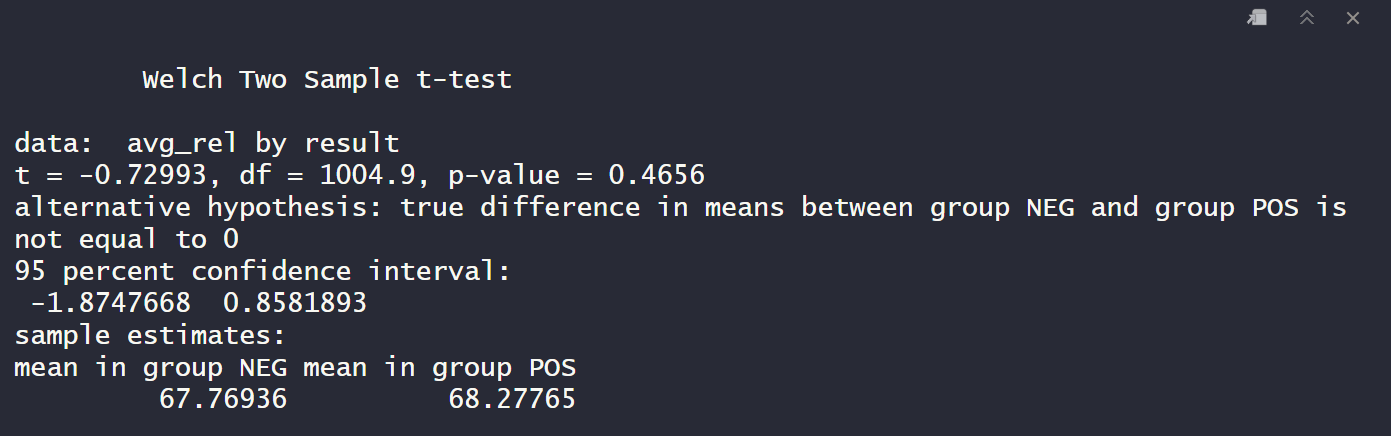
\includegraphics{images/Screenshot 2023-12-15 162220.png}

}

\caption{t-test conducted on average relative humidity and test results}

\end{figure}

Based on the results of the t-test, the p-value when testing average
temperature was far bellow 0.05, meaning that there is a statistically
significant relationship between temperature and mosquito test results
and that we cam reject the null hypothesis. However, for relative
humidity, the high p-value of 0.46 means that there is not a
statistically significant relationship between relative humidity and
test result. From the calculated confidence interval, it shows that I am
95\% confident that the impact of temperature on test results falls
within the range of (-3.4, -2.4).

\hypertarget{linear-regression-summary}{%
\subsubsection{Linear Regression
Summary}\label{linear-regression-summary}}

Following this, i conducted a linear regression on both tests to further
unpack the atmospheric influence on mosquito test results.

\begin{figure}

{\centering 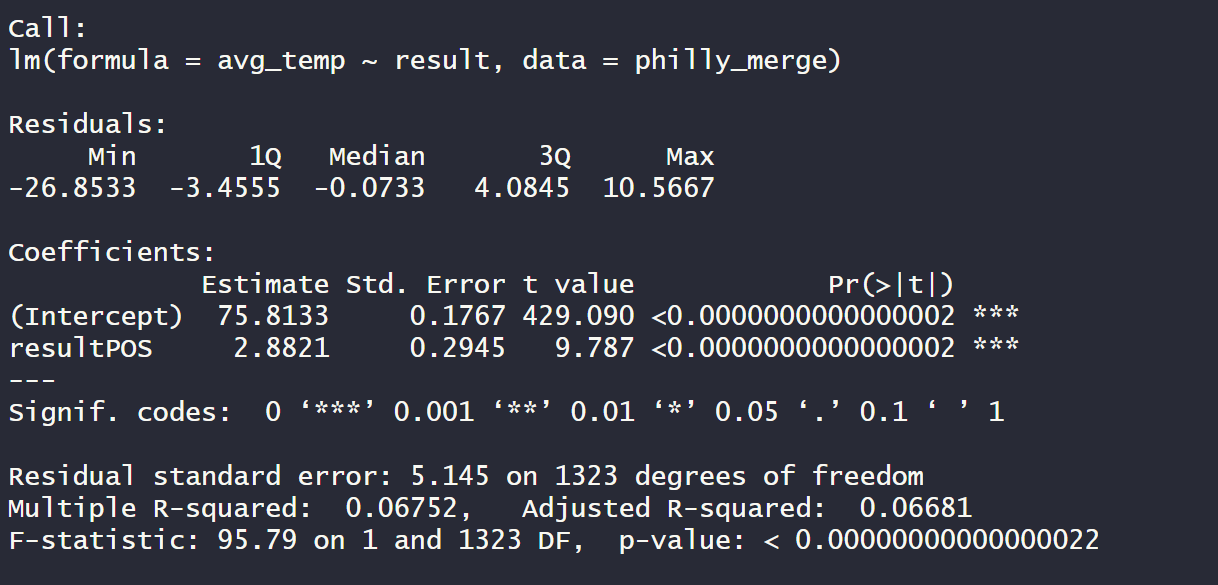
\includegraphics{images/Screenshot 2023-12-15 162303.png}

}

\caption{Linear model on average temperature and test results}

\end{figure}

\begin{figure}

{\centering 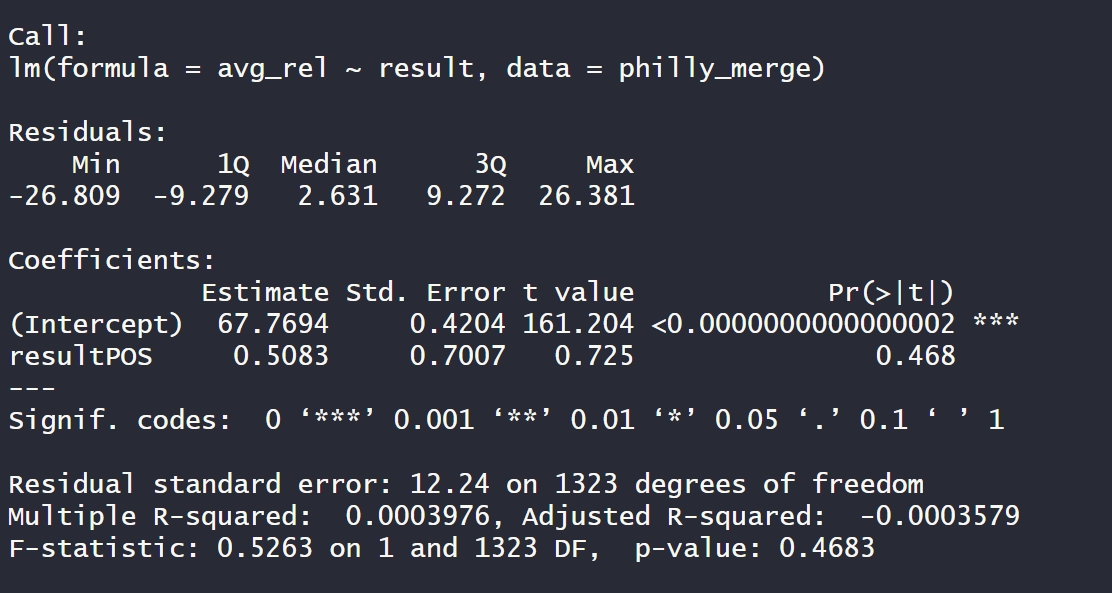
\includegraphics{images/Screenshot 2023-12-15 162349.png}

}

\caption{Linear model on average relative humidity and test results}

\end{figure}

From the table shown above, it can be concluded that for every 1 degree
increase in temperature, the positive test results will increase by 2.
It also shows that at 0, the average temperature is approx. 75 degrees.
It can also be concluded that for every 1\% increase in relative
humidity, positive test results will increase by 0.5. And that at 0, the
average relative humidity is approx. 67\%. The R-squared value for
temperature is .066, meaning that 6\% of the positive test results could
be explained by average temperature. For relative humidity, the
R-squared value is -0.0003, meaning that none of the test results could
be explained by average relative humidity.

\hypertarget{time-series-analysis}{%
\subsection{Time Series Analysis}\label{time-series-analysis}}

Since research showed that mosquito populations within Philadelphia have
been increasing over the years due to higher average temperatures with
each year, I wanted to explore this relationship in addition to the
analysis conducted above. I conducted a time series analysis on both
Philadelphia mosquito counts in 2018 and Philadelphia mosquito counts
from the entire range of the data set, 2001-2020. I initually wanted to
explore the relationship between time and mosquito test results, however
I had difficulty in doing so due to the test result data being binary.
The following figures show my results.

\begin{figure}

{\centering 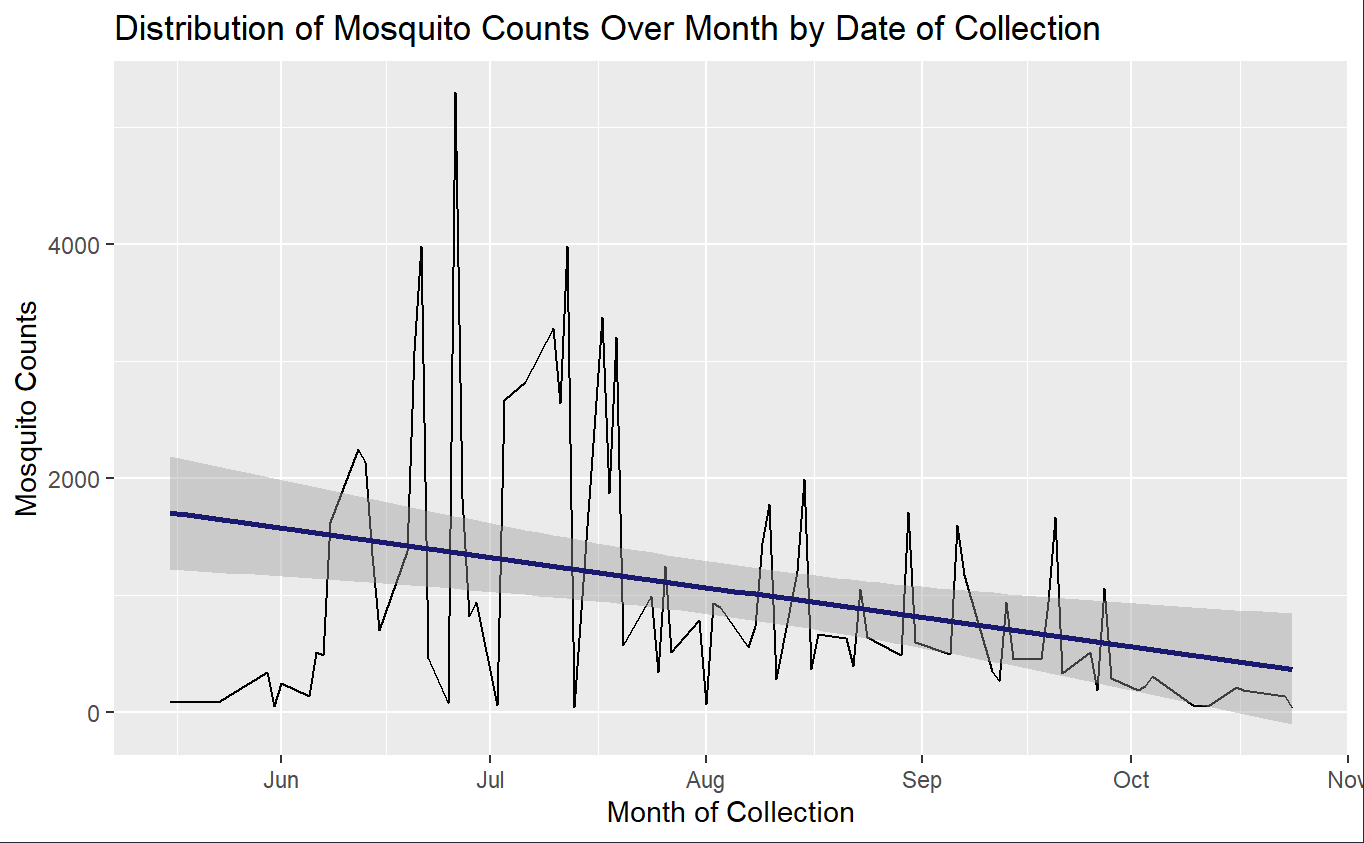
\includegraphics[width=8.33333in,height=\textheight]{images/ts_by_day.png}

}

\caption{Fig. 3 Time series analysis of Philadelphia Mosquito Counts by
Date of Collection in 2018. The results show a downward trend in
mosquito counts as they thrive in warmer temperatures seem during the
spring and summer}

\end{figure}

I first plotted a basic analysis and regression of mosquito counts over
the months of May - October per day of collection. The output (Fig 3.)
showed that there is a downward trend in mosquito counts by month, which
is expected since mosquitoes tend to me most active during warmer
months. There is also evidence of a spike in mosquito counts near the
end of June.

Following this, I converted the data into a time series object and
conducted a decomposition, breaking the analysis down into ``trend'' and
``noise.'' Since the data was only collected over a year, there was no
seasonality found. The results of the decomposition are as follows.

\begin{figure}

{\centering 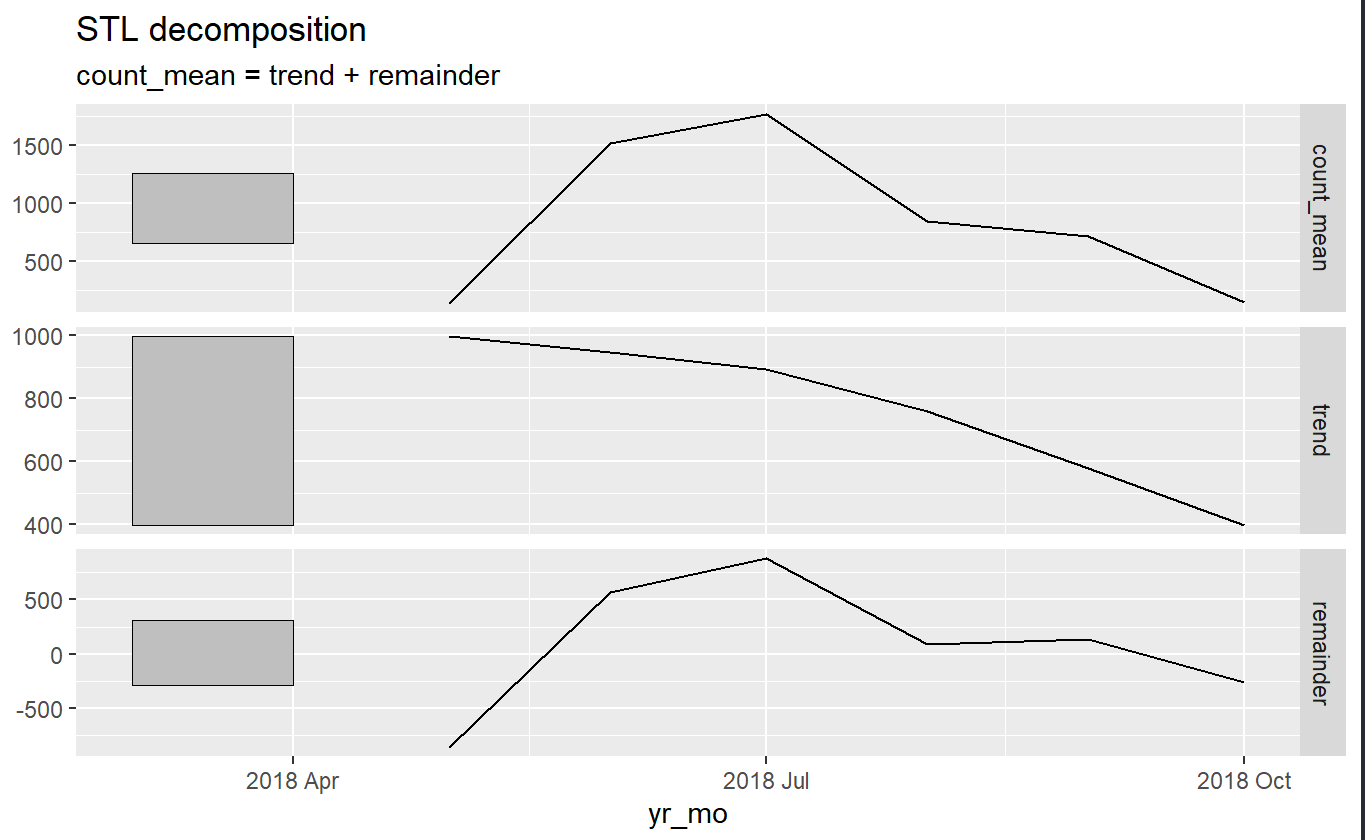
\includegraphics{images/decomp_components.png}

}

\caption{Fig. 4 A time series decomposition of mosquito counts over May
2018 and October 2018, showing the trend in counts and remainders}

\end{figure}

The bars on the left side of the graph (Fig. 4) help to compare the
magnitude of the cycles. The bar for trend is quite large, indicating
that it likely not important in driving the mosquito counts.

(Fig. 5) was produced as a result of the decomposition, plotting the
adjusted data

\begin{figure}

{\centering 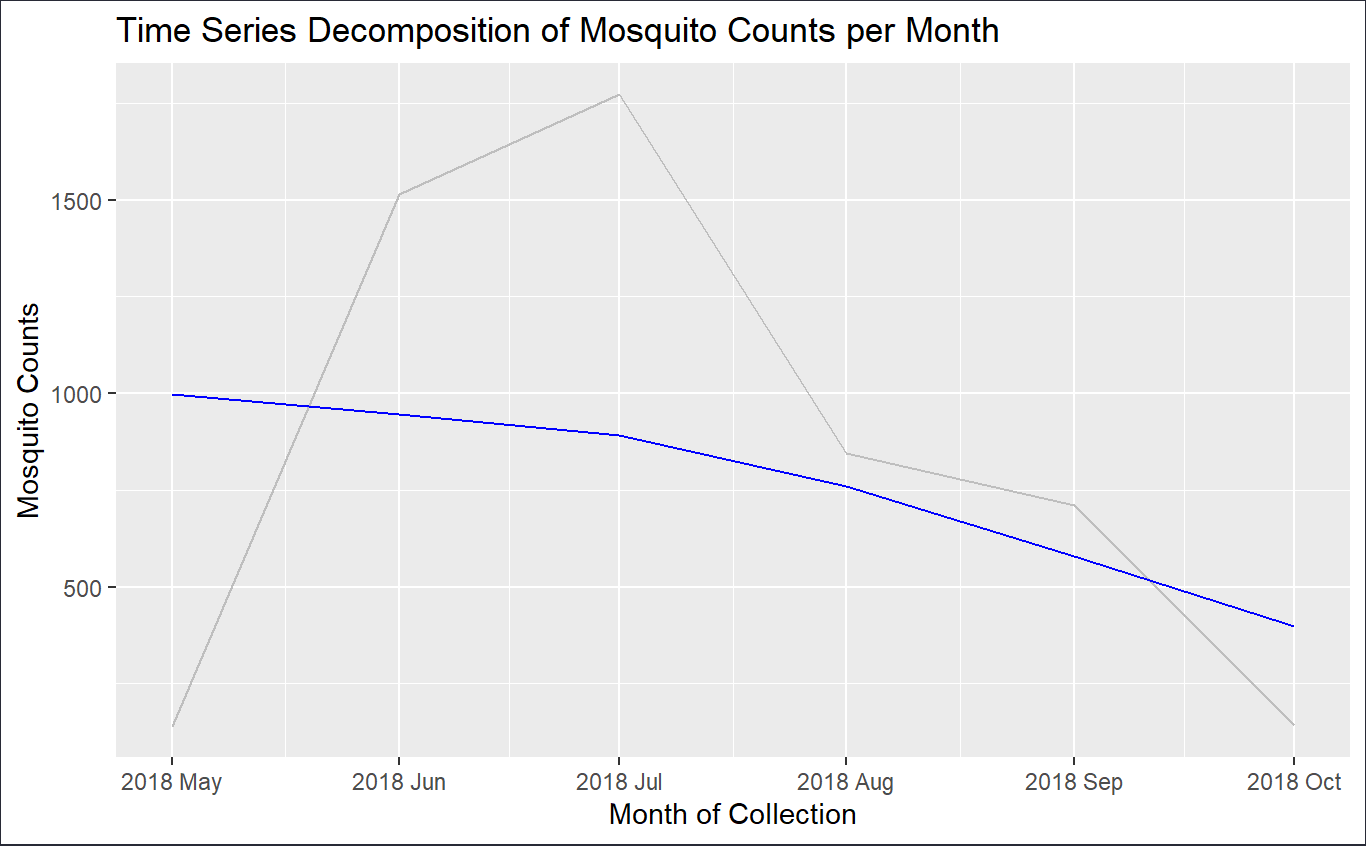
\includegraphics{images/Screenshot 2023-12-15 155208.png}

}

\caption{Fig. 5 Adjusted time series analysis of mosquito counts by
month of collection}

\end{figure}

The results of this analysis show a spike in mosquito counts in July
followed by a sharp decreased in counts throughout the rest of the
collection period. Since this analysis only looked at one year of data,
I decided to look at the entire mosquito collection cycle (2021 - 2020)
within Philadelphia

\begin{figure}

{\centering 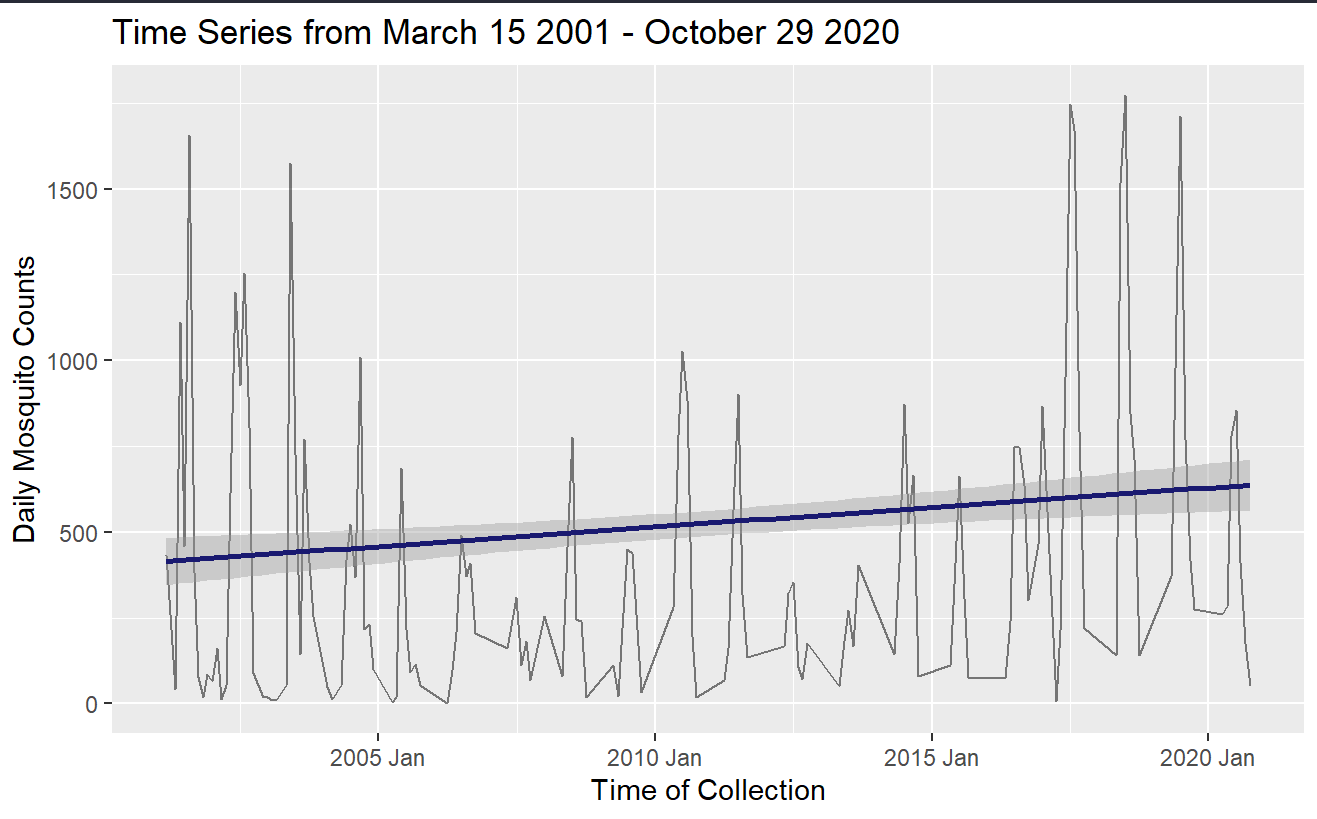
\includegraphics[width=8.33333in,height=\textheight]{images/full_time_series-01.png}

}

\caption{Fig. 6 Basic time series of mosquito counts from start of
series collection (March 2001) to end of series collection (September
2020). The regression line shows a positive trend in mosquito counts
over the years that has been steadily increasing since 2001.}

\end{figure}

This plot (Fig.6) shows that there is a positive trend in mosquito
counts throughout the years of collection, possibly due to increases in
temperature making Philadelphia a much more habitable place for
mosquitoes for a longer period of time. To follow up on these results
and to find if there was a significant seasonal trend in the data, I
attempted a decomposition. However, due to the significant amount of
gaps in time from the months of collection starting and ending at
different times per year and there being several days throughout the
periods where there was no collection (resulting in the error ``internal
NA's''), I was unable to do a deeper exploration of the time series.

\hypertarget{future-analysis-and-conclusions}{%
\section{Future Analysis and
Conclusions}\label{future-analysis-and-conclusions}}

Based on the tests conducted, it is reasonable to believe that there is
a connection between average temperature and positive mosquito test
results, however, that may not be the only factor in influencing the
relationship. I believe that further analysis is needed to definitively
determine if atmospheric factors like temperature impact the amount of
mosquitoes that test positive for West Nile Virus. Including other
variables like the cases of WNV in birds, collection locations (vacant
lots, parks, neighborhoods, etc) and other weather events such as
flooding would help to determine a more concrete relationship in what
determines both the count of mosquitoes and the occurrence of WNV in
populations.

Additionally, having a more detailed data set that details whether or
not the test results were for the entire population of mosquitoes tested
in that location, for that day, or for an individual mosquito in that
population would be beneficial.

\hypertarget{references}{%
\section{References}\label{references}}

Hook, J. (2018, October 9). \emph{Pennsylvania is having its worst
outbreak of West Nile virus in 15 years}. Public Opinion.
https://www.publicopiniononline.com/story/news/2018/10/09/pennsylvanias-worst-outbreak-west-nile-virus-15-years/1580572002/

Kummer, F. (2020, August 4). \emph{Mosquitoes arrive earlier, stay later
in Philly region because of climate change, data suggest}.
https://www.inquirer.com.
https://www.inquirer.com/science/climate/mosquitos-climate-change-climate-central-global-warming-philadelphia-allentown-atlantic-city-zika-20200804.html

\emph{Mosquitoes}. Department of Environmental Protection. (n.d.).
https://www.dep.pa.gov/Business/ProgramIntegration/Vector-Management/Mosquitoes/Pages/default.aspx

ssadowski@pennlive.com, S. S. \textbar. (2018, August 7). \emph{West
Nile hot spots in Pa.: What\textquotesingle s The risk in your county?}
pennlive.
https://www.pennlive.com/news/erry-2018/08/94f441765f7887/west-nile-hot-spots-in-pa-what.html



\end{document}
